
\section{Measuring charge transport}

Transport measurements have been performed for over a century now and was the technique by which superconductivity was first discovered. The relative technical simplicity of the measurements makes transport measurements highly appealing considering the wealth of information that they can provide about a material.

The charge transport measurements performed for this thesis took place in Bristol in the Green `Polo' magnet and also in Toulouse for the high field data. The six-probe measurement technique is the same for all the transport measurements with only slight adjustments between Hall and magnetoresistnace measurements.

\subsection{Experimental apparatus}

\subsubsection{Six probe technique}

For accurate measurement of voltage, and hence resistance, across a sample, two wires are not sufficient. The wires themselves have a resistance which would also be summed inot the measurement. A solution to this problem is to instead supply the current for the voltage reading via one set of wires, and then take the voltage reading from another set meaning that a minimum of four wires and four contacts on the sample are required. To measure magnetoresistance we require the voltage wires to be placed upstream and downstream of the current, to measure the Hall effect we require the wires to be placed transverse to the current. Moreover it is useful to be able to take two transport measurements at a time so as to get an idea for the homogeneity of the sample and as well to provide some redundancy in case of breakage. Since the \BSCO samples that we studied were to have both measurements, six connection points were placed to each sample as shown in figure~\ref{Fig:Exp:BSCOSampleSchematic}.
\begin{figure}[htbp]
    \begin{center}
        \includegraphics[scale=0.9]{Chapter-ExperimentalTechnique/Figures/BSCOSampleSchematic/BSCOSampleSchematic}
        \caption{An example \BSCO crystal mounted on the quartz substrate. Voltage legs are labeled a, b, c and d.}
        \label{Fig:Exp:BSCOSampleSchematic}
    \end{center}
\end{figure}
The connections were made with \unit[20]{$\mu m$} gold wire for the current and \unit[10]{$\mu m$} gold wire for the voltage leads and attached with DuPont 4929 silver paint which dries at room temperature. As shown in the figure, the sample is raised from the quartz substrate \TODO{Why is the sample raised?}.

With the four voltage legs a variety of configurations can be achieved. Measureing across (a) and (b) is the magnetoresistance configuration, (a) and (c) is the Hall configuration. It is also possible to measure across (a) and (d) and provided the field is reveresed from positive to negative, both the Hall and the magnetoresistance across the sample can be extracted.

Because the connections may not be exactly aligned and because the silver paint in practice covers a relatively large area of the sample, magnetoresistance contributions may be found in the Hall configuration and vise-versa. For this reason it is generally advised to sweep both with a positive field to obtain $R_{\textrm{pos}}$ and a negative field to obtain $R_{\textrm{neg}}$ where $R$ is the resistance and separate the two out using,
\begin{align}
R_{\textrm{Hall}} &= \frac{1}{2}( R_{\textrm{pos}} - R_{\textrm{neg}} ) \\
R_{\textrm{MR}} &= \frac{1}{2}( R_{\textrm{pos}} + R_{\textrm{neg}} )
\end{align}



\subsubsection{Polo magnet}

\subsubsection{High field laboratory, Toulouse}

\subsection{Sample size determination}

\subsection{Data Analysis}

\subsubsection{Field lag correction}

